  \section{Introduction}
    \bframe
      \begin{block}<1-2>{Problématique}
        \begin{itemize}
          \item architecture NUMA
          \item systèmes non efficaces
          \item gain de performances
        \end{itemize}
      \end{block}
      \begin{block}<2>{Objectifs}
        \begin{itemize}
          \item évaluation d'activité
          \item mesures d'évènements
        \end{itemize}
      \end{block}
    \end{frame}

  \section{Architecture NUMA}
    \subsection{Présentation}
      \bframe
        \begin{columns}[T]
          \begin{column}{.5\textwidth}
          \begin{block}{Objectifs}
            \begin{itemize}
              \item accélerer les temps de traitement
              \item répondre aux besoins d'applications spécifiques
            \end{itemize}
          \end{block}
          \begin{block}{Moyens mis en \oe uvre}
            \begin{itemize}
              \item découpe en noeuds
              \item placement des contrôleurs d'E/S
              \item liens d'interconnexions
              \item mise en place d'une topologie
            \end{itemize}
          \end{block}
        \end{column}
        \begin{column}{.5\textwidth}
          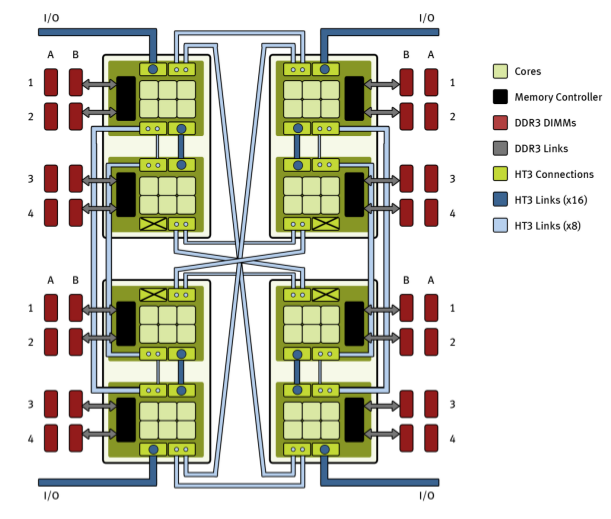
\includegraphics[scale=0.4]{img/numa_arch_details.png}
        \end{column}
      \end{columns}
    \end{frame}

    \subsection{Enjeux}
      \bframe
        \begin{itemize}
          \item placement mémoire
          \item placement des threads
          \item activité d'entrées/sorties
        \end{itemize}
        \myfig{0.4}{img/topo.png}
      \end{frame}

  \section{Infrastructure de tests}
    \subsection{}
      \bframe
        \begin{block}<1-2>{}
          \begin{itemize}
            \item utilisation mutualisée du Magny Cour $\rightarrow$ machines
              virtuelles
            \item compilation du noyau avec KGDB
            \item problème: aucune émulation du monitoring par Qemu
          \end{itemize}
        \end{block}
        \begin{alertblock}<2>{Conséquence}
          \begin{itemize}
            \item Travail en réel sur le noyau pour 50\% du projet
          \end{itemize}
        \end{alertblock}
      \end{frame}


